\section{密度的计算}
\label{sec:dens-computation}

前几节回答了密度何时存在、怎样使用。本节回到两类具体对象：可数集合上由点质量给出的测度，以及实轴上由累积函数的增量给出的测度。每个例子都按同一顺序处理：先固定参考测度，检查绝对连续性，再求密度，最后代入换测度公式核对它能否恢复目标测度的质量与积分。

\subsection{离散测度的密度}
\label{sec:dens-discrete}

可数集合上每个点都可以单独称量，所以离散测度的密度可以逐点计算，这是向量类比完全成立的情形。需要分别处理的只是参考质量为零的点。

\paragraph{点质量之比}
设$X=\{x_1,x_2,\ldots\}$是可数集合，取全部子集为可测集，参考测度与目标测度分别为
\[
\mu=\sum_im_i\delta_{x_i},\qquad\nu=\sum_ip_i\delta_{x_i},\qquad m_i,p_i\in[0,+\infty).
\]
单点质量有限，可数个单点覆盖$X$，所以两者都$\sigma$有限。

先检查绝对连续。$\mu(A)=0$当且仅当$A$中每点的$m_i$都为零，所以$\nu\ll\mu$当且仅当“$m_i=0$推出$p_i=0$”。在此条件下令
\begin{equation}
h(x_i)=\frac{p_i}{m_i}\quad(m_i>0),\qquad h(x_i)\ \text{取任意非负值}\quad(m_i=0).
\label{eq:dens-discrete}
\end{equation}

对离散测度的积分是加权求和，于是对任意$A\subset X$，
\[
\begin{aligned}
\int_Ah\,\mathrm d\mu&=\sum_{x_i\in A}h(x_i)m_i=\sum_{x_i\in A,\,m_i>0}p_i\\
&=\sum_{x_i\in A}p_i=\nu(A),
\end{aligned}
\]
第三个等号用到$m_i=0$时$p_i=0$。所以$h$是$\nu$相对于$\mu$的密度。

两类点的处理不同。参考质量为正的点上，密度值就是质量之比，被唯一确定。参考质量为零的点构成$\mu$零测集，密度在那里可以任意取值，这正是几乎处处版本在离散情形的样子。以计数测度为参考时所有$m_i=1$，密度就是目标的点质量本身，即概率质量函数。

\paragraph{参考零测点上的目标质量}
若某点$m_i=0$而$p_i>0$，不能用“取一个很大的有限比值”来补救：任何有限或无限的$h(x_i)$都满足$h(x_i)m_i=0\neq p_i$。这时的问题不在于比值难算，而在于$\nu\ll\mu$不成立，密度根本不存在。

正确的做法是先作Lebesgue分解。令$N=\{x_i:m_i=0\}$，则$\nu$的奇异部分与绝对连续部分分别是
\[
\nu_{\mathrm s}=\sum_{x_i\in N}p_i\delta_{x_i},\qquad\nu_{\mathrm{ac}}=\sum_{x_i\notin N}p_i\delta_{x_i} ,
\]
只有$\nu_{\mathrm{ac}}$才有密度$p_i/m_i$。

例如在$X=\{0,1,2\}$上取
\[
\mu=\delta_0+\delta_1,\qquad\nu=\tfrac12\delta_0+\tfrac14\delta_1+\tfrac14\delta_2 ,
\]
则$N=\{2\}$，点$2$上的质量$\tfrac14$是奇异部分。$\nu_{\mathrm{ac}}$的密度在$0,1$处分别为$\tfrac12,\tfrac14$。

\begin{example}[同一分布换两种参考]
\label{ex:dens-poisson}
在$\{0,1,2,\ldots\}$上取参数为$1$的Poisson分布$p_k=\mathrm e^{-1}/k!$为目标。相对于计数测度，密度就是$p_k$本身。若改用几何权重$m_k=2^{-(k+1)}$作参考，所有$m_k>0$，密度为
\[
h(k)=\frac{p_k}{m_k}=\frac{2^{k+1}\mathrm e^{-1}}{k!} .
\]
前六项约为
\[
0.736,\quad1.472,\quad1.472,\quad0.981,\quad0.491,\quad0.196 .
\]
核对集合$\{0,1\}$的质量。直接求和与加权求和分别是
\[
\begin{aligned}
\nu(\{0,1\})&=2\mathrm e^{-1}\approx0.7358,\\
h(0)m_0+h(1)m_1&\approx0.7358\cdot0.5+1.4715\cdot0.25\approx0.7358 ,
\end{aligned}
\]
两者一致。两种密度由链式规则联系：几何权重相对于计数测度的密度是$m_k$，所以$h(k)\cdot m_k=p_k$。
\end{example}

图~\ref{fig:dens-discrete}画出了两组点质量及它们的比值。比值大于$1$的地方，目标比参考更重；$k$增大后几何权重比阶乘倒数衰减得慢，比值趋于零。

\begin{BookInlineFigure}
  \centering
  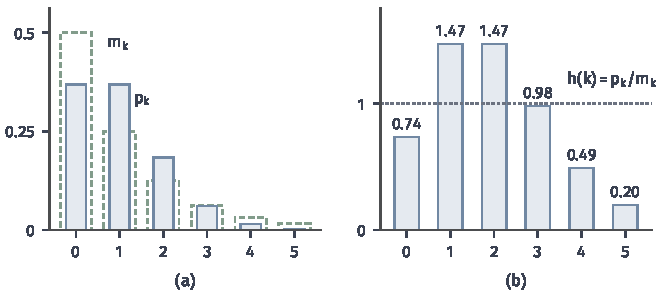
\includegraphics[width=112mm]{figures/04-spaces-measures-and-geometry/02-measure/matplotlib/dens-discrete/figure.pdf}
  \caption{可数集合上的离散密度。(a)绿色虚线框为几何参考质量$m_k=2^{-(k+1)}$，蓝色柱为Poisson目标质量$p_k=\mathrm e^{-1}/k!$，$k=0,\ldots,5$。(b)密度$h(k)=p_k/m_k$：$k=1,2$处目标质量相对参考最多，$h$约为$1.47$；$k$增大后$h$趋于零。}
  \label{fig:dens-discrete}
\end{BookInlineFigure}

密度的计算与总质量是否有限无关。仍以几何权重为参考，计数测度$\sum_k\delta_k$的密度是$h(k)=2^{k+1}$，目标的总质量为$+\infty$，但每个集合上的质量都由$h$正确恢复。代入换测度公式，例如对$f(k)=k$，
\[
\sum_kk\,p_k=\sum_kk\,\frac{p_k}{m_k}\,m_k ,
\]
两边都是Poisson分布的均值$1$。

\subsection{由累积函数求密度}
\label{sec:dens-cumulative-density}

实轴上的测度常常由累积函数给出。设$F:\mathbb R\to\mathbb R$单调不减且右连续，第~\ref{chap:measure}章的Stieltjes构造给出Borel测度$\mu_F$，满足$\mu_F((s,t])=F(t)-F(s)$。它在每个有界区间上有限，因而$\sigma$有限。我们要问$\mu_F$何时有Lebesgue密度，以及密度怎样从$F$算出。

\begin{theorem}[累积函数的密度]
\label{thm:dens-cumulative}
设$F:\mathbb R\to\mathbb R$单调不减且右连续。
\begin{enumerate}
\item 若$F$在每个有界闭区间上绝对连续，则$\mu_F\ll\lambda$，并且
\begin{equation}
\frac{\mathrm d\mu_F}{\mathrm d\lambda}=F'\qquad\lambda\text{几乎处处}.
\label{eq:dens-cumulative}
\end{equation}
\item 反之，若$\mu_F\ll\lambda$，则$F$在每个有界闭区间上绝对连续。
\end{enumerate}
\end{theorem}

\begin{proof}
(1) 由第~\ref{chap:integration}章，绝对连续函数几乎处处可导，导数局部可积，并且
\[
F(t)-F(s)=\int_s^tF'(x)\,\mathrm dx .
\]
$F$单调不减，在可导点差商非负，所以$F'\geq0$几乎处处，可以取非负版本。

令$\nu(A)=\int_AF'\,\mathrm d\lambda$。由定理~\ref{thm:dens-weighted-measure}它是测度，并且在每个区间$(s,t]$上与$\mu_F$相等。两者在每个$(-m,m]$上有限；半开区间族对交封闭并生成Borel $\sigma$代数，由第~\ref{chap:measure}章测度延拓的唯一性，$\nu=\mu_F$。于是$F'$是$\mu_F$相对于$\lambda$的密度，$\mu_F\ll\lambda$。

(2) 固定$[a,b]$。$\lambda$是$\sigma$有限的，由Radon–Nikodym定理存在非负可测$h$使$\mu_F(A)=\int_Ah\,\mathrm d\lambda$，并且
\[
\int_a^bh\,\mathrm dx=F(b)-F(a)<\infty .
\]
于是对$x\in[a,b]$，
\[
F(x)=F(a)+\mu_F((a,x])=F(a)+\int_a^xh(t)\,\mathrm dt .
\]
可积函数的变上限积分绝对连续，所以$F$在$[a,b]$上绝对连续。
\end{proof}

定理把函数的绝对连续与测度的绝对连续联系起来：对单调累积函数，“总长度小的区间组上增量之和小”恰好对应“长度零测集上没有增量质量”。密度就是导数，但只在几乎处处意义下确定：$F$在个别点上可以没有导数，在那里给密度取什么值都不影响$\mu_F$。

\begin{example}[多项式累积函数]
\label{ex:dens-square-cdf}
令$F(x)=0$（$x<0$），$F(x)=x^2$（$0\leq x\leq1$），$F(x)=1$（$x>1$）。$F$在每个有界闭区间上是Lipschitz的，因而绝对连续，于是$\mu_F$相对于$\lambda$的密度是
\[
F'(x)=2x\mathbf 1_{(0,1)}(x).
\]
在$x=1$处$F$没有导数，但单点不影响密度。代入换测度公式，
\[
\int x\,\mathrm d\mu_F=\int_0^1x\cdot2x\,\mathrm dx=\tfrac23 ,
\]
与第~\ref{sec:dens-change-of-measure}小节的例子一致。
\end{example}

\paragraph{检查原子与奇异连续部分}
定理的条件不能省略，也不能只检查$F$是否连续。计算一般累积函数的密度时，应当按第~\ref{sec:dens-decomposition}节的分解逐项检查。第一步读出跳跃：由式~\eqref{eq:dens-jump}的同一推导，$F(x)-F(x-)=\mu_F(\{x\})$，跳跃点就是原子。第二步去掉跳跃后检查余下的连续部分是否绝对连续；若是，它的导数就是$\mu_F$的绝对连续部分的密度，否则还有奇异连续部分。只把$F'$当作整个测度的密度，会同时漏掉这两类质量。

\begin{example}[有跳跃的累积函数]
\label{ex:dens-mixed-cdf}
令
\[
F(x)=\begin{cases}0,&x<0,\\\tfrac12+\tfrac x2,&0\leq x<1,\\1,&x\geq1.\end{cases}
\]
$F$在$0$处从$0$跳到$\tfrac12$，其余处连续，所以$\mu_F$有原子$0$，质量$\tfrac12$。去掉跳跃后的$F-\tfrac12\mathbf 1_{[0,\infty)}$在$[0,1]$上是$\tfrac x2$，绝对连续，导数$\tfrac12$。于是
\[
\mu_F=\tfrac12\delta_0+\tfrac12\lambda|_{[0,1]} ,
\]
只有后一项有Lebesgue密度$\tfrac12\mathbf 1_{[0,1]}$。

用换测度公式检验差别。取$g(x)=1+x$，正确的积分把原子和密度两部分都算上：
\[
\int g\,\mathrm d\mu_F=\tfrac12g(0)+\int_0^1\tfrac12(1+x)\,\mathrm dx=\tfrac12+\tfrac34=\tfrac54 .
\]
若误把$F'$当作整个测度的密度，只得到
\[
\int_0^1(1+x)\cdot\tfrac12\,\mathrm dx=\tfrac34 ,
\]
恰好漏掉原子贡献的$\tfrac12g(0)=\tfrac12$。
\end{example}

图~\ref{fig:dens-cumulative-jump}左边是累积函数，右边是它对应的测度。左图的跳跃高度变成右图的箭头，左图的斜率变成右图的密度。

\begin{BookInlineFigure}
  \centering
  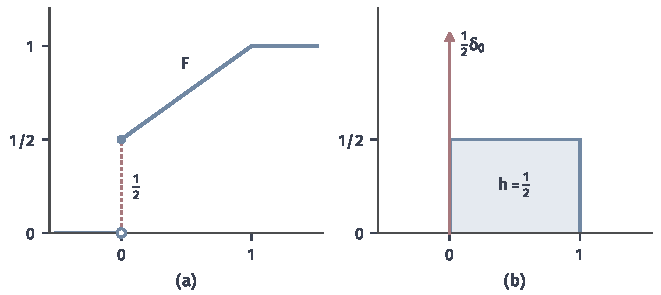
\includegraphics[width=112mm]{figures/04-spaces-measures-and-geometry/02-measure/matplotlib/dens-cumulative-jump/figure.pdf}
  \caption{有跳跃的累积函数与它的测度。(a)$F$在$0$处跳跃$\tfrac12$（红色虚线），在$(0,1)$上斜率为$\tfrac12$。(b)对应的测度$\mu_F=\tfrac12\delta_0+\tfrac12\lambda|_{[0,1]}$：红色箭头是原子，蓝色区域是密度$\tfrac12$表示的连续质量。}
  \label{fig:dens-cumulative-jump}
\end{BookInlineFigure}

连续却不绝对连续的情形由Cantor函数给出。第~\ref{sec:dens-real-line-decomposition}小节的混合例子中，去掉跳跃后的$\tfrac x2+\tfrac14F_C(x)$已经连续，却仍有$\tfrac14$的奇异连续质量，其导数几乎处处等于$\tfrac12$，只恢复绝对连续部分。所以“$F$连续”“$F$几乎处处可导”都不足以让导数成为整个测度的密度，必须要求绝对连续。

对右连续的有界变差函数，增量可以为负。这时可以先写成两个单调函数之差，再对两个Stieltjes测度分别应用本小节的步骤，最后按有限有符号测度的规则相减。
